%% This is the main file and you use this file to organize your assignment.

\documentclass[a4paper]{article}	  
\usepackage[margin=3cm]{geometry} 	   % Choose your margin here. 
\usepackage{amsmath}
\usepackage{parskip}
\usepackage{graphicx}
\usepackage{caption}
\usepackage{subcaption}
\usepackage{todonotes}
\DeclareMathOperator{\sgn}{sgn}

\newcommand{\figref}[1]{\figurename~\ref{#1}}

\let\endtitlepage\relax						% Begin the text immidiately after the title page. Optional
\setlength{\parindent}{0cm}				% Start paragraph without indent. Optional

\begin{document}

\begin{titlepage}
\begin{center}
\Large TTK4190 Guidance and Control of Vehicles \\
\vspace{10pt}
\Large  Assignment 2 \\
\vspace{10pt}
\large Written Fall 2018 By \\
\large Anders Haver Vagle,\\ Ada Skarsholt Larsen,\\ Sondre Aleksander Bergum,\\ Martin Madsen
\begin{figure}[h]
\centering
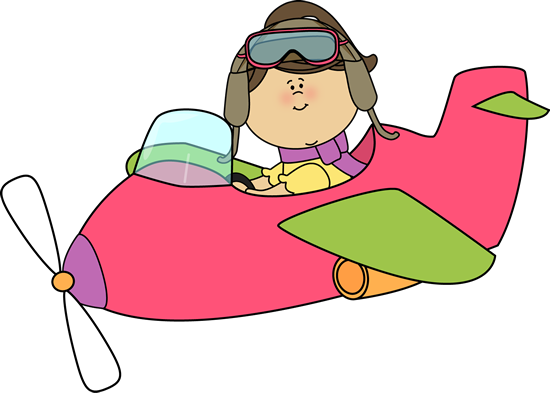
\includegraphics[width=0.5\textwidth]{flying-plane-clipart.jpg}
\end{figure}

\begin{figure}[b]
\centering

\includegraphics[width=0.5\textwidth]{itk_ntnu}\\
Department of Engineering Cybernetics
\end{figure}
\end{center}
\end{titlepage}



\section*{Problem 1 - Attitude Control of Satellite}

\subsection*{Problem 1 a)} 

\textbf{What is the ground speed of the aircraft (numerical value) in the absence of wind?} \\
In the absence of wind, $V_w = 0$, we have $V_g = V_a = 580 km/h$.

\subsection*{Problem 1 b)}

\textbf{Write down two expressions for the sideslip (crab) angle $\beta$ in the absence of wind. One expression should depend on aircraft velocity and the other on aircraft heading.} \\

\begin{align}
    \beta &= \sin^{-1}\left( \frac{v_r}{\sqrt{u_r^2 + v_r^2+w_r^2}}\right ) \\
    \beta &= \chi_c - \psi
\end{align}

\subsection*{Problem 1 c)}

\textbf{Compute the Dutch-roll natural frequency and relative damping ratio for the aircraft. Can you,
very briefly with your own words, describe how the Dutch roll mode affect the yaw and roll
motion? How would the motion change with increased relative damping ratio?}

\begin{align}
    \lambda_{dutch-roll} = \frac{Y_v+N_r}{2 }\pm \sqrt{\left(\frac{Y_v+N_r}{2}\right)^2 - \left(Y_vN_r - N_vY_r\right)}
\end{align}

With the constants found from the state space model 

\begin{align}
    Y_V = -0.322 \\ 
    N_R = -0.32 \\
    N_V = 0.0426 \\
    Y_R = -180.44
\end{align}
We get 

\begin{align}
    \lambda = -0.321 \pm 2.77i \\
    \omega_n = 2.79 \\
    \zeta = 0.1147
\end{align}

Dutch roll will affect roll and yaw by inducing an oscillation in yaw which is "transferred" to roll. If you increase the damping ratio the oscillation will dampen faster. 


\subsection*{Problem 1 d)}

\textbf{Compute the spiral-divergence mode. Is the mode unstable?} \\
For the spiral-divergence mode we assume that $\dot{\bar{p}} = \Bar{p} = 0$ and that the rudder command is negligible. We have
\begin{align}
    \lambda_{spiral} &= \frac{N_rL_v - N_vL_r}{L_v} 
\end{align}

With the constants

\begin{align}
    L_v = -0.0657 \\
    L_r = 0.46
\end{align}

We get \\
\begin{align}
    \lambda_{spiral} = -0.022
\end{align}

Since $\lambda$ is less than 0 we do not have an unstable mode. 

\subsection*{Problem 1 e)}
\textbf{Compute the roll mode. Is the roll mode faster or slower than the spiral-divergence mode?} \\
We can find the roll mode by ignoring the heading dynamics and assuming a constant pitch angle. An approximation of the eigenvalue for the rolling mode is given by  
\begin{align}
    \lambda_{roll} &= L_p \\
    &= -2.87
\end{align}
This mode is faster, as the pole is more negative.


% Note that \mathbf can be used for bold letters in math mode (within equations and dollar signs). \boldsymbol can be used to get bold greek letters.  	% Use "\include" instead of "\input" if you want the section to start on a new page. "problem1" is a tex file included at this location in the document. It is possible to answer the whole assignment in the main file (paste everything from "problem1.tex" and "problem2.tex" here), but that restricts the readability. Therefore, one file is created for each problem.
\section*{Problem 2 - Autopilot for course hold using aileron and successive loop closure}
\subsection*{Problem 2 a)}
\textbf{Find numerical values for $a_{\phi_1}$
and $a_{\phi_2}$ based on the state-space model.}


\begin{align}
    \delta_a\left(\frac{a_{\phi_2}}{s+a_{\phi_1}}\right) = p \quad &\Rightarrow \quad \frac{p}{\delta_a} = \frac{a_{\phi_2}}{s+a_{\phi_1}} \\
    \dot{p} &= -10.6\beta - 2.87p + 0.46r -0.65\delta_a \\
    \dot{p} &= -2.87p - 0.65\delta_a \\
    \Rightarrow p(s+2.87) &= -0.65\delta_a \\
    \Rightarrow \frac{p}{\delta_a} &= -\frac{0.65}{s+2.87}
\end{align}

Therefore

\begin{align}
    a_{\phi_1} = 2.87 \\
    a_{\phi_2} = -0.65 
\end{align}

\subsection*{Problem 2 b)}

\textbf{Find numerical values for the five gains $k_{p\phi}$, $k_{d\phi}$, $k_{i\phi}$, $k_{i\chi}$, and $k_{p\chi}$.} \\

First we find the control gains of the inner loop which control roll angle and roll rate. \\
We find the control gains $k_{p\phi}$ and $k_{d\phi}$ based on the desired response of the closed-loop dynamics. The transfer function from $\phi^c$ to $\phi$ is given by

\begin{align}
    H_{\phi/\phi^c}(s) = \frac{k_{p_\phi}a_{\phi_2}}{s^2 + (a_{\phi_1} + a_{\phi_2}k_{d_\phi})s + k_{p_\phi}a_{\phi_2}}
\end{align}

This can be recognized as the canonical second-order transfer function 

\begin{align}
    \frac{\phi(s)}{\phi^c(s)} = \frac{\omega^2_{n_\phi}}{s^2+2\zeta_\phi \omega_{n_\phi}s+\omega^2_{n_\phi}}
\end{align}

If we then equate the denominator polynomial coefficients we get

\begin{align}
    \omega^2_{n_\phi} &= k_{p_\phi}a_{\phi_2} \\
    2\zeta_\phi \omega_{n_\phi} &= a_{\phi_2} + a_{\phi_2}k_{d_\phi} \\
\end{align}

The proportional gain is selected so that the ailerons saturate when the roll error is $e^{max}_\phi$ where $e^{max}_\phi$ is a design parameter. Therefore we get 

\begin{align}
   k_{p\phi} &= \frac{\delta_a^{max}}{e_{\phi}^{max}}\sgn(a_{a_{\phi2}}) \\
   &= -\frac{30}{15} \\
   &= -2
\end{align}

The $\delta_a^{max}$ is the maximum deflection of the ailerons. The natural frequency of the roll loop is therefore given by

\begin{align}
    \omega_{n\phi} &= \sqrt{|a_{\phi2}|\frac{\delta_a^{max}}{e_{\phi}^{max}}} = \sqrt{1.3} \\
\end{align}

Which gives

\begin{align}
    k_{d\phi} &= \frac{2\zeta_{\phi}\omega_{n\phi}-a_{\phi1}}{a_{\phi2}} \\
    &= \frac{2\cdot 0.707 \cdot \sqrt{1.3} - 2.87}{-0.65} \\
    &= 1.935
\end{align}

Where the damping ratio $\zeta_{\phi}$ is a design parameter given as $\zeta_{\phi}= 0.707$. \\

An integrator is then added to the loop which gives a new transfer function 

\begin{align}
    H_{\phi/\phi^c}(s) = \frac{k_{p_\phi}a_{\phi_2}\left( s + \frac{k_{i_\phi}}{k_{p_\phi}}\right)}{s^3 + (a_{\phi_1} + a_{\phi_2}k_{d_\phi})s^2 + k_{p_\phi}a_{\phi_2}s + k_{i_\phi}a_{\phi_2} }
\end{align}

Since $a_{\phi_2}$ and $a_{\phi_1}$ is known, $k_{i_\phi}$ can be effectively selected using root locus techniques. The closed-loop poles of the system are given by 

\begin{align}
    1 + k_{i_\phi} \left(\frac{a_{\phi_2}}{s(s^2 + (a_{\phi_1} + a_{\phi_2}k_{d_\phi})s + k_{p_\phi}a_{\phi_2})} \right) = 0 
\end{align}

\begin{figure}[h!]
    \centering
    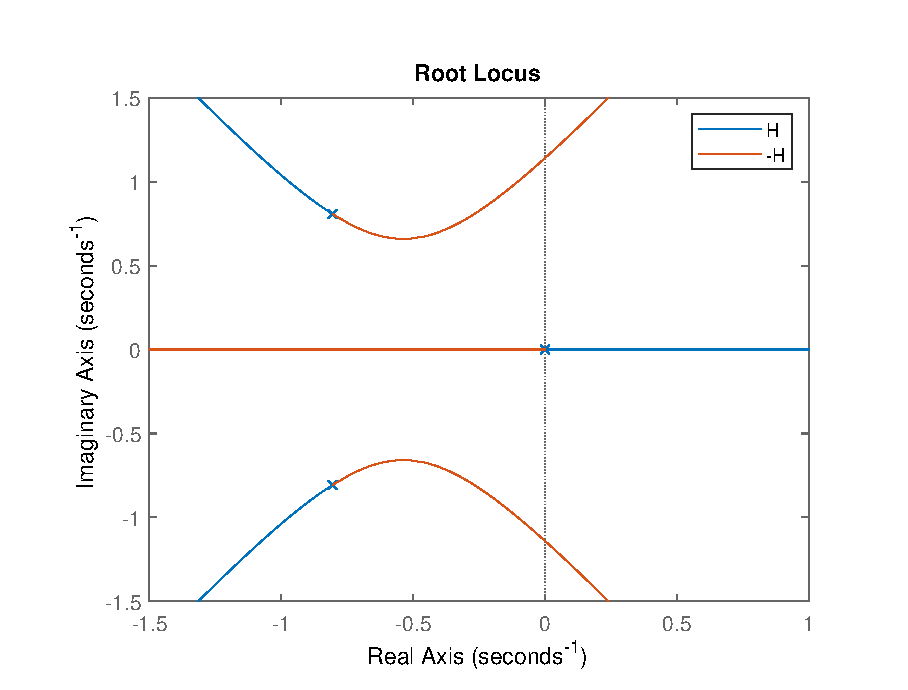
\includegraphics[width=\textwidth]{rootlocus.eps}
    \caption{Root locus analysis}
    \label{fig:root_locus}
\end{figure}

From the root locus analysis in fig. \ref{fig:root_locus} we see that no $k_{i\phi} > 0$ results in all poles being in the left half-plane. For all three poles to be stable, we should choose:

\begin{align}
    -3 < k_{i\phi} \leq 0
\end{align}


We find that choosing $ k_{i\phi} = 0$, thereby entirely removing the integral gain, gives the best results. This is discussed further in the next subtask. 



To find the course-hold gains we look at the outer loop assuming that the inner loop has been adequately tuned such that $H_{\phi/\phi^c} \approx 1$. Using the transfer function $H_{\chi}$ given by

\begin{align}
    H_{\chi} = \frac{2\zeta_{\chi}\omega_{n_{\chi}}s + \omega^2_{n_{\chi}}}{s^2 + 2\zeta_{\chi}\omega_{n_{\chi}}s + \omega^2_{n_{\chi}}}
\end{align}

We use the natural frequency and damping to find the final two gains.

\begin{align}
    \omega_{n_{\chi}} &= \frac{1}{W_{\chi}} \omega_{n_{\phi}} \\
    k_{p_{\chi}} &= 2\zeta_{\chi}\omega_{n_{\chi}}V_g/g \\
    k_{i_{\chi}} &= \omega^2_{n_{\chi}}V_g/g 
\end{align}

The inner loop needs to be at least 5-10 times faster than the outer loop. This is achieved by setting the bandwidth separation $W_{\chi}$. Through a number of simulations, we found that $\zeta_{\chi} = 1.8$ and $W_{\chi}= 18$ gives the best response. This gives gains

\begin{align}
    \omega_{n_{\chi}} = 0.063 \\
    k_{p_{\chi}} = 3.725 \\
    k_{i_{\chi}} = 0.065 \\
\end{align}

\subsection*{Problem 2 c)}

We already have an integral action in the outer course loop. This is typically sufficient, and so we should be able to achieve stability without any integral action in the inner roll loop. Also, we need the inner loop to be significantly faster than the outer loop. The integral will add both delay and instability, and thus we figure we are better of without it. This was confirmed by testing various values for $k_{i_{\phi}}$, seeing no improvement caused by the integrator.


\subsection*{Problem 2d)}

We have the maneuver 

\begin{align}
    \chi_{ref} = 
    \begin{bmatrix}
    0 & 10 & -5 & -10 & 5 & 10 & 20 & 20 \\
    \end{bmatrix}
\end{align}

With time vector

\begin{align}
    t = 
    \begin{bmatrix}
    0 & 60 & 140 & 230 & 300 & 380 & 500 & 600 \\
    \end{bmatrix}
\end{align}

Which gives the simulation results seen in figure \ref{fig:response_2d}. Our autopilot is kind of slow, taking about 80-90 seconds to reach the desired course after a step of up to 15 degrees. However, a too fast response would be uncomfortable for the passengers of the plane. It is also assumed that the plane would not have to change course very frequently on a typical flight, meaning the extra seconds for stabilization are perfectly acceptable.

\begin{figure}[!h]
    \centering
    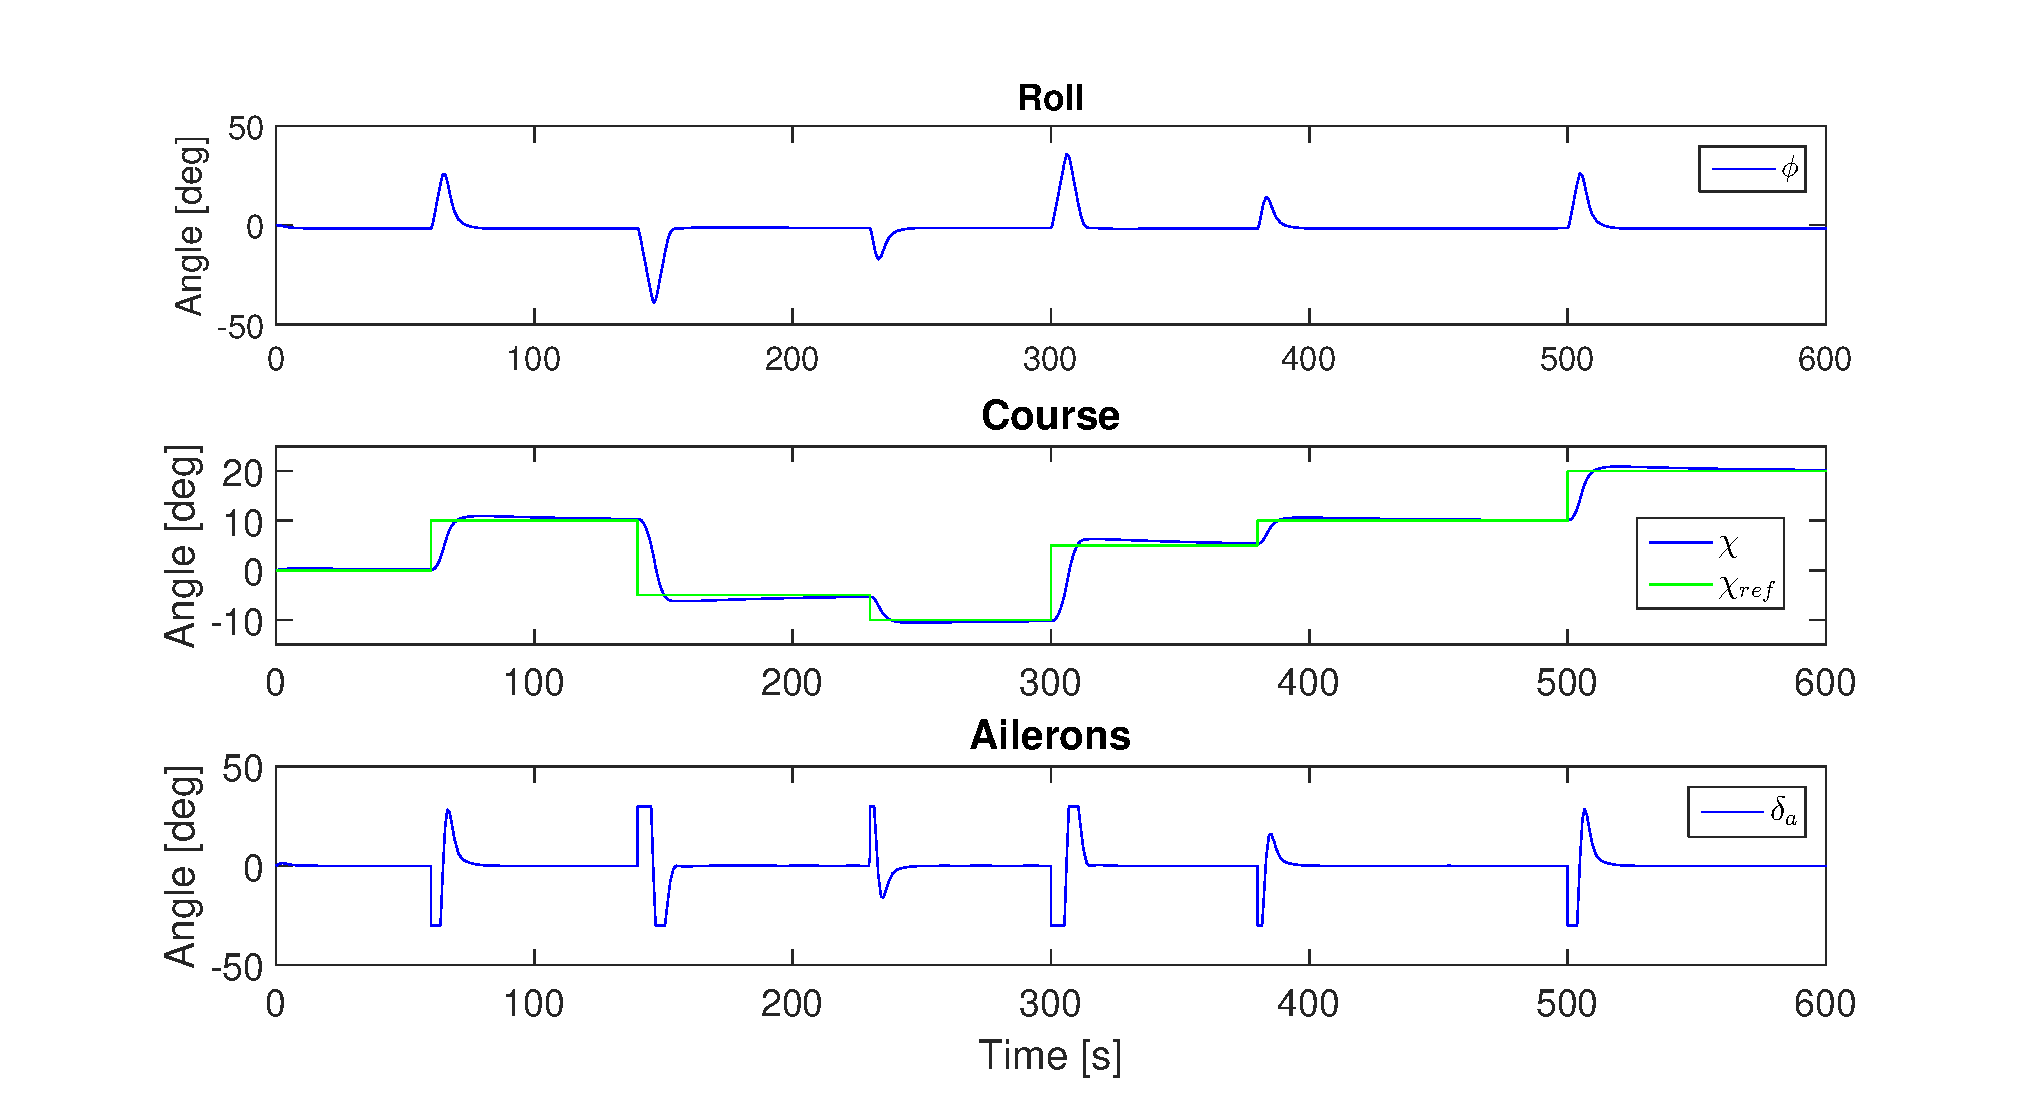
\includegraphics[width=\textwidth]{prob2d.eps}
    \caption{Roll, course inputs and response and aileron inputs for simplified model}
    \label{fig:response_2d}
\end{figure}

We see that the ailerons reach saturation for a few seconds at each change in course reference, but overall the response is smooth.


\subsection*{Problem 2e)}

\begin{figure}
    \centering
    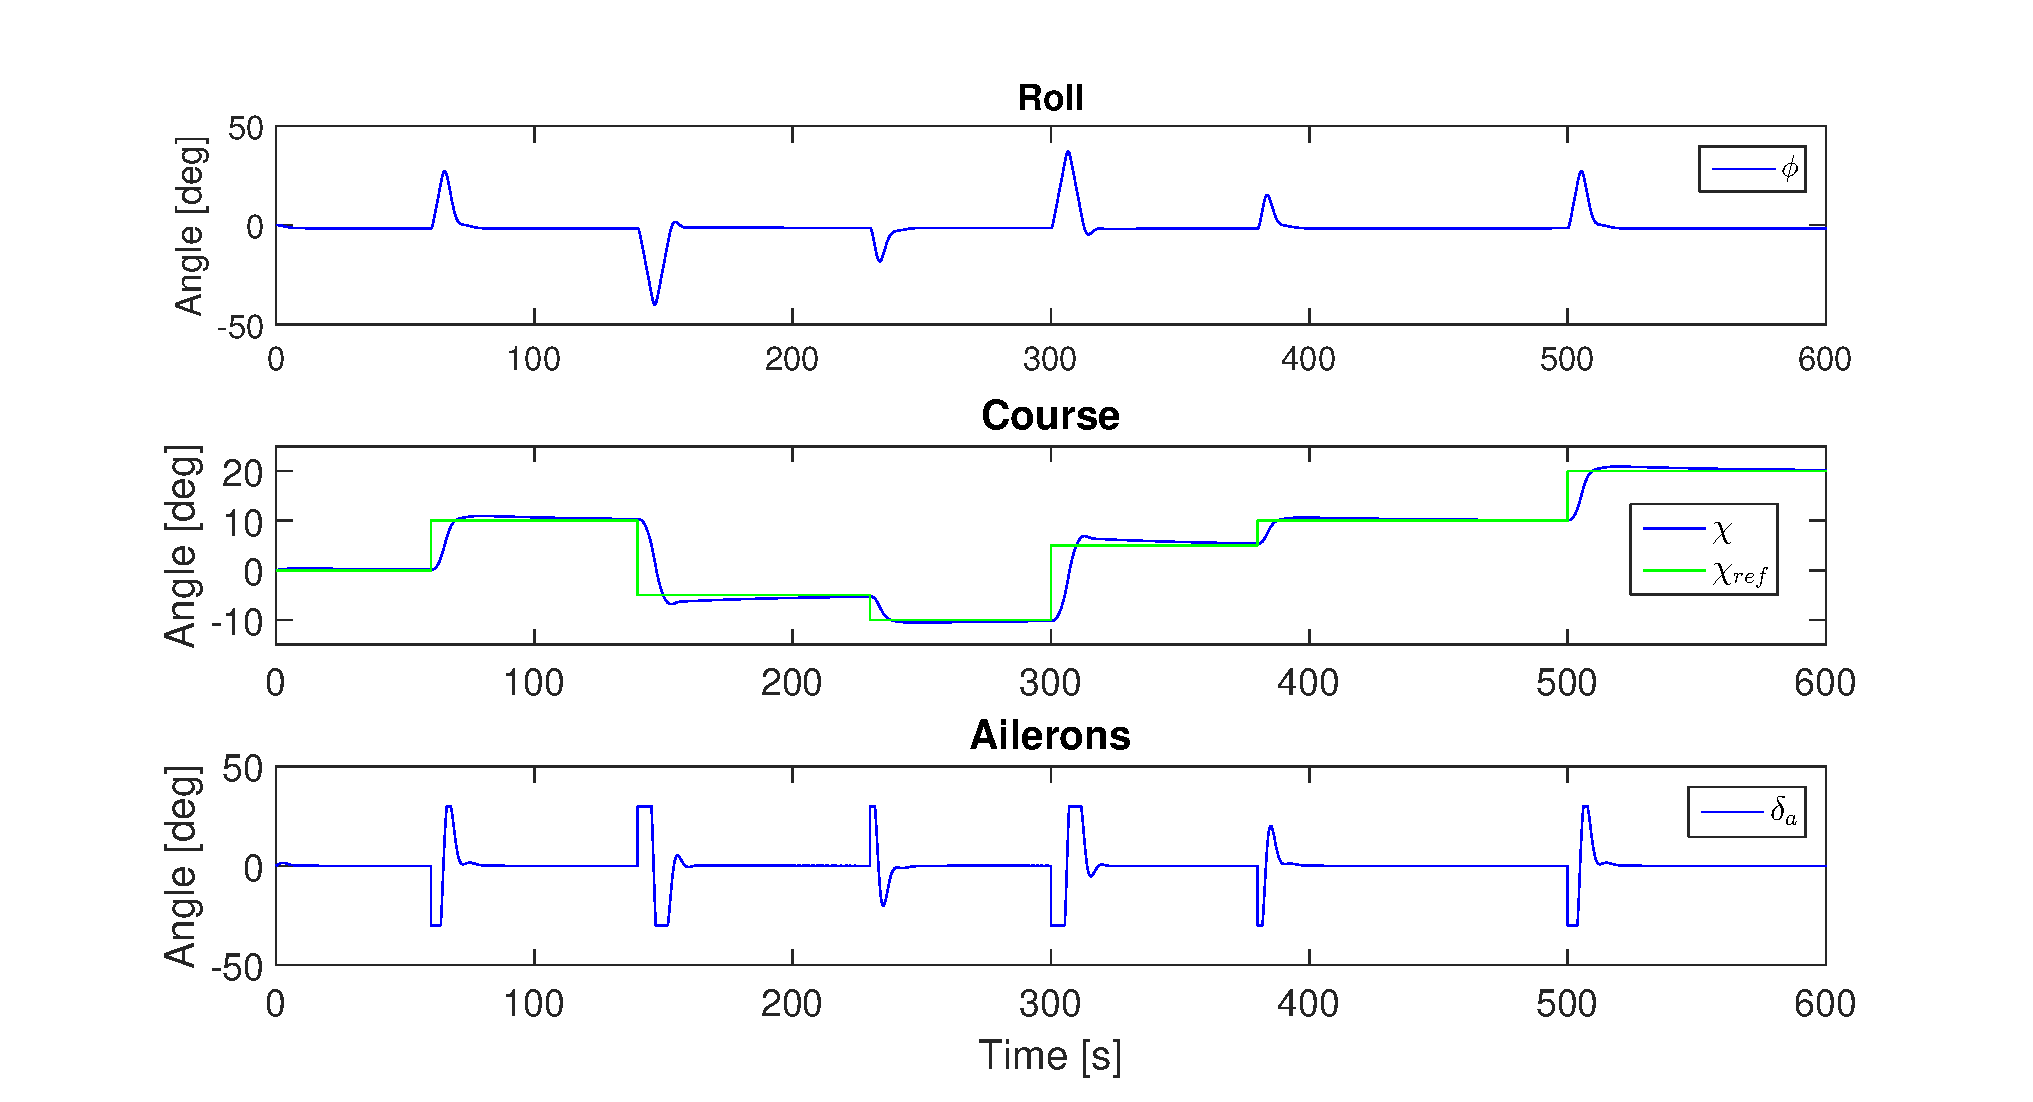
\includegraphics[width=\textwidth]{prob2e.eps}
    \caption{Roll, course inputs and response and aileron inputs for real dynamics}
    \label{fig:response_2e}
\end{figure}

Comparing figure \ref{fig:response_2d} and figure \ref{fig:response_2e}, we see very little difference. Figure \ref{fig:response_2e}, based on the state-space model, shows slightly more oscillations and overshoot than the simplified model, but the performance is still satisfactory. This indicates that the simplified model is a good approximation for the true dynamics. There are only some minor errors in the transient response. 

\subsection*{Problem 2f)}

Wind-up occurs whenever the aileron input is saturated. By looking at our results we find that when this happens there is a slight overshoot. Though it is not very significant, we implemented an anti-windup scheme to see if we improve performance.
This solution handles the problem by using the inputs exceeding saturation limits as an added term in the integrator gain, scaled by its own gain $k_{aw}$. The input to the integrator then becomes:

\begin{align}
    k_{i_{\chi}}+k_{aw}*(\delta_{a, unsat}-\delta_{a, sat}) \\
\end{align}

We found from testing that the value of $k_{aw}=0.02$ yields performance slightly better than without the anti-windup effect. This can be seen in figure \ref{fig:response_2f}. Here, a comparison is made between the anti-windup being active and inactive. There is noticeably less overshoot in the course angle with anti-windup, meaning its inclusion is validated.

\begin{figure}
    \centering
    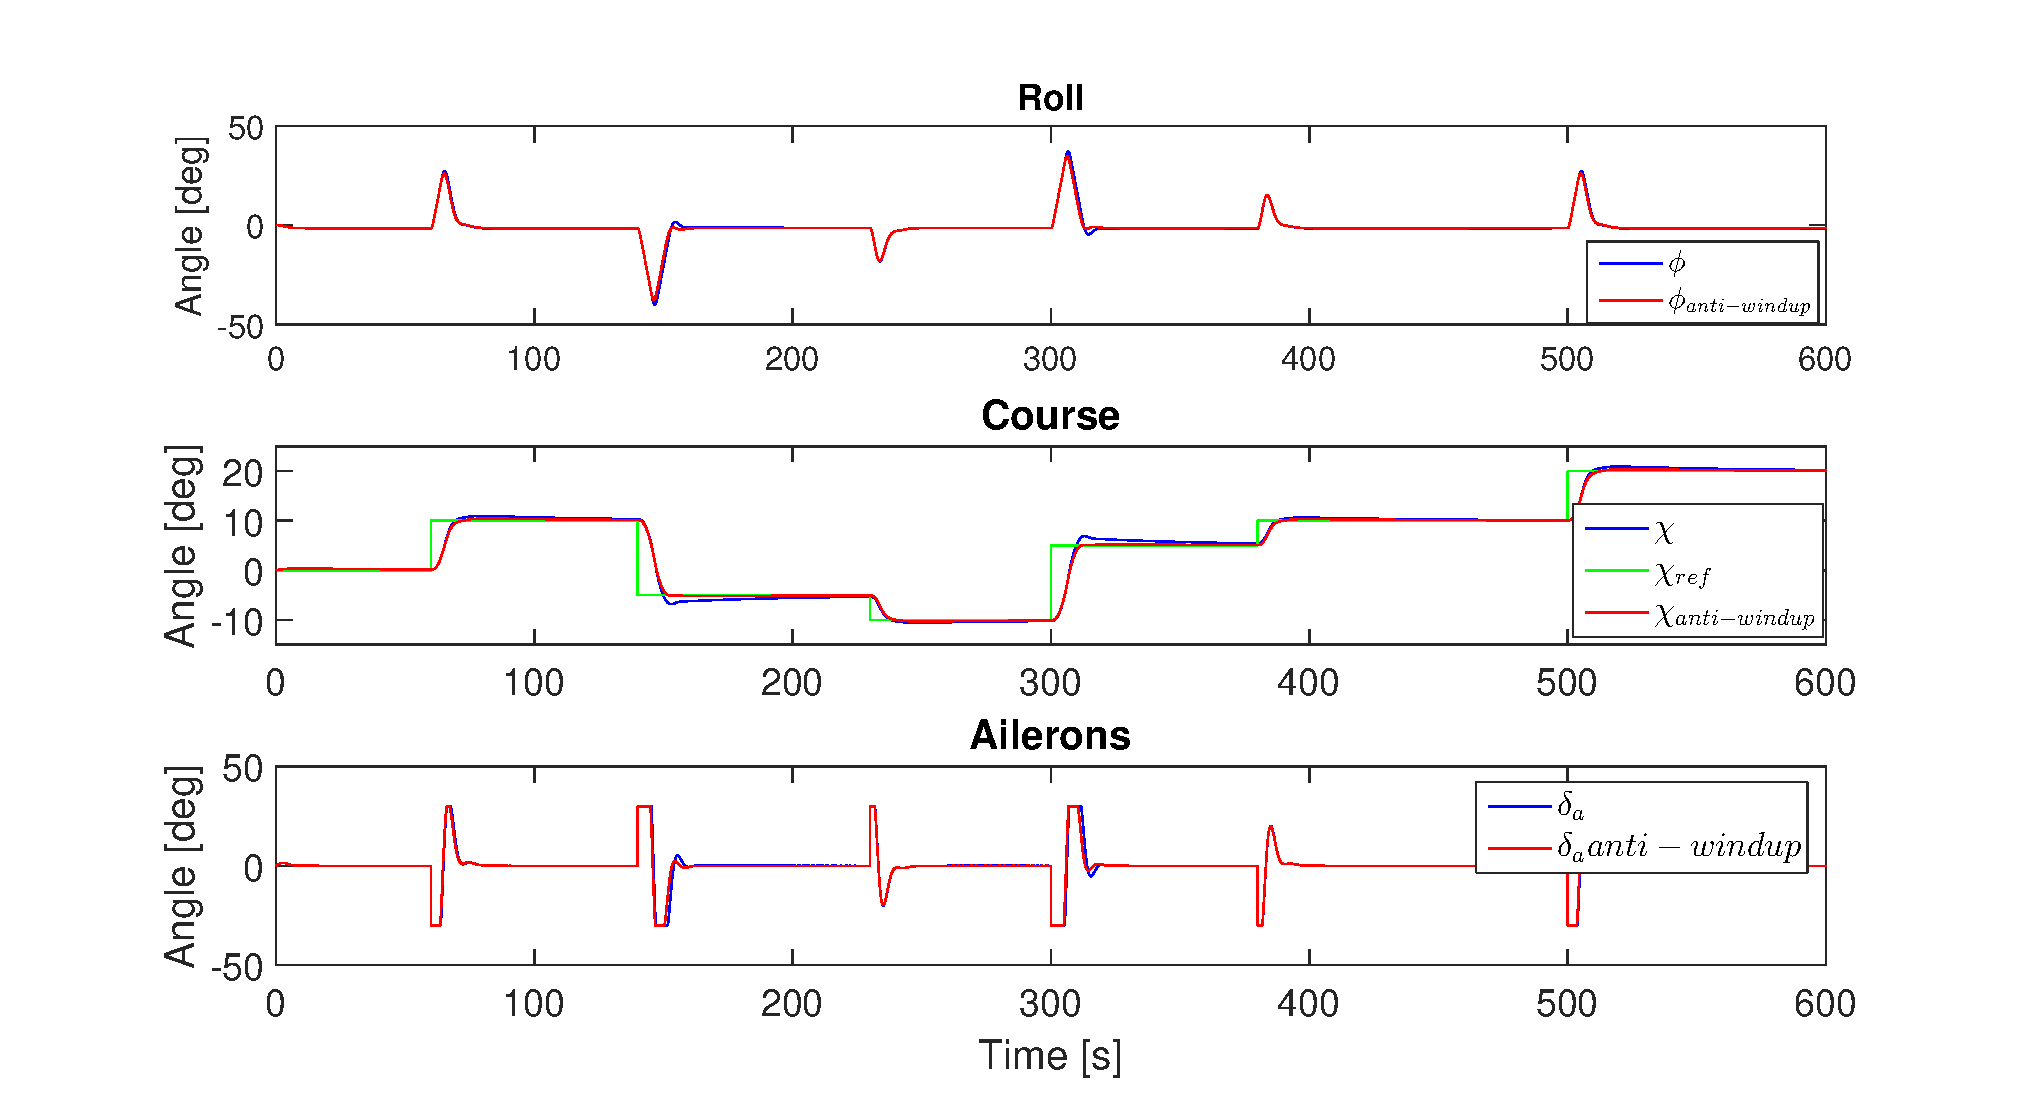
\includegraphics[width=\textwidth]{prob2f.eps}
    \caption{Roll, course inputs and response and aileron inputs for real dynamics with and without anti-windup}
    \label{fig:response_2f}
\end{figure}

 
%\bibliographystyle{IEEEtran}
%\bibliography{bibliography.bib}

\end{document}